% 
% Annual Cognitive Science Conference
% Sample LaTeX Paper -- Proceedings Format
% 

% Original : Ashwin Ram (ashwin@cc.gatech.edu)       04/01/1994
% Modified : Johanna Moore (jmoore@cs.pitt.edu)      03/17/1995
% Modified : David Noelle (noelle@ucsd.edu)          03/15/1996
% Modified : Pat Langley (langley@cs.stanford.edu)   01/26/1997
% Latex2e corrections by Ramin Charles Nakisa        01/28/1997 
% Modified : Tina Eliassi-Rad (eliassi@cs.wisc.edu)  01/31/1998
% Modified : Trisha Yannuzzi (trisha@ircs.upenn.edu) 12/28/1999 (in process)
% Modified : Mary Ellen Foster (M.E.Foster@ed.ac.uk) 12/11/2000
% Modified : Ken Forbus                              01/23/2004
% Modified : Eli M. Silk (esilk@pitt.edu)            05/24/2005
% Modified : Niels Taatgen (taatgen@cmu.edu)         10/24/2006
% Modified : David Noelle (dnoelle@ucmerced.edu)     11/19/2014

%% Change "letterpaper" in the following line to "a4paper" if you must.

\documentclass[10pt,letterpaper]{article}
\usepackage{standalone}
\usepackage[dvipsnames]{xcolor}
\usepackage{sty/mypackages}
\usepackage{tkz-euclide}

\AtBeginDocument{\renewcommand{\APACrefYearMonthDay}[3]{\BBOP{#1}\BBCP}}

\usepackage[ruled,vlined]{algorithm2e}
\usepackage{url}

\usepackage[%
%font={small,sf},
labelfont=bf,
format=hang,
format=plain,
margin=0pt,
%width=0.8\linewidth,
]{caption}
\usepackage[list=true, font={normalsize}]{subcaption}

\usepackage{silence}
%Disable all warnings issued by latex starting with "You have..."
\WarningFilter{latex}{You have requested package}

\DeclareMathOperator*{\argmax}{argmax}



\newcommand{\TODO}[1]{\textcolor{red}{\Large{#1}}}
\newcommand{\module}[1]{\textcolor{black}{\texttt{#1}}}

\title{Inverse Planning as a Framework for Insect Navigation Research}
 
\author{{\large \bf Paulina Friemann (friemanp@cs.uni-freiburg.de)} \\
  Department of Computer Science, \\
  University of Freiburg}

\begin{document}

\maketitle

\iffalse
\todo{i get now where this should be going: overall question of which pathfinding algos are there, how biologically plausible are they? two paths: 1) theoretical work of things like time and memory complexity, representational structures, performance (?), (dis-)advantages, assumptions and constraints, etc. 2) experimental sampling in a framework: explanation of the framework, what is there etc., then frame it as okay we want to take a look at not only this value iteration policy generation, but at all kinds of pathfinding algos, adapted to solve the same problem, i.e., to generate policies over the environment. here we can build the bridge towards trajectory sampling stuff.}
\fi

\begin{abstract}
The study of insect navigation is a very active field of research.
Computational modeling approaches mainly focus on the simulation of behavior observed in experiments.
In this project, a framework is proposed based on inverse planning, taking inspiration from a cognitive model of goal inferences in human subjects.
In this framework, computational models can be embedded, and either be used as grounds for sampling data, or as a comparison to experimental data.
The Bayesian frame allows to draw numerical inferences to agent goals or to the models themselves.
\end{abstract}

\iffalse
\begin{itemize}
	\item Introduction
	\item Tenenbaum Paper
	\item Problem Definition....from Pathfinding to Policy Finding
	\item Pathfinding Algos
	\item Program Workings, pseudocode and formulas
	\item Trajectory Sampling
\end{itemize}
\fi


%\todo{Bounded Rationality; also Iris van Roi stuff whatsitcalled}

\todo{Composite Decision Process Kumar and Kanal 1988}

\todo{Pseudocodes Basic Algos}

\todo{Probabilistic interpretation of heuristics Handsson and Mayer 1989}

\todo{How to do A* / heuristic based algos if we want policies? I think it's actually ok to just not expand the nodes, and only do it if the trajectory actually does it, so only in the posterior calculation, not in the policy calculation}

\todo{trajectory sampling}

\todo{
	Value Iteration
	One iteration takes O(|A||S|2) time.
	• Number of iterations required :
	poly(|S|,|A|,1/(1-$\gamma$))
	• Overall, the algorithm is polynomial in state
	space, and thus exponential in number of
	state variables
}

\todo{Branch and Bound (Lawler and Wood 1966 for survey); Minimum-Spanning-Tree Heuristic (Held and Karp 1970)}

\todo{For policies: Need to solve all pairs shortest paths? -> dynamic programming and memoization. Bob Floyd1962a, 1962b; Karger et al. 1993}

\todo{How to connect policies with pathfinding algos? --> see trajectory sampling?}

\todo{we use regular grid representation, however, there are others (see \cite{algfoor2017})}

\todo{Exploration Exploitation}
\todo{Space \& time complexity}


\section{Introduction}

% general intro
% pathfinding (AI, biologically inspired, models)
% Path1 & Path2 explanations
% related works
% structure

The modeling of movement of biological agents is an active research field \cite<c.f. e.g.,>{lemoel2020a, webb2016}.
Computational models can support the discovery of biological mechanisms underlying a specific skill, help to discern between different theories, and propose new experiments to further develop existing theories.
Models can furthermore be used to make assumptions explicit, and discover limitations and restrictions to theories and methods.
Moreover, they can aid in exploring internal variables which cannot be measured directly, such as internal representations of perceived external information.

Many insights from biological agents' ways of solving problems have been used in research on Artificial Intelligence (AI; \citeNP{darwish2018}).
Theories, such as the path integration strategy found in some insects \cite<cf.,>{heinze2018b, wehner2009} have been applied for example in biologically-inspired mobile robots \cite<e.g.,>{lambrinos2000, weber1999}.
Oftentimes, these applications take inspiration from abstract perspectives on biologically implemented skills (for a recent overview, see \citeNP{darwish2018}, and \citeNP{agarwal2020}, for a review specifically for robot navigation).
These biologically-inspired algorithms are then optimized for a specific purpose, such as application, and computational or memory simplicity, and rather ignorant to the biological counterpart,
which is especially illustrated by the application of swarm optimization techniques for path-finding of single agents \cite<cf.,>{agarwal2020}, and hopes to hybridize different bio-inspired algorithms \cite{fan2020, darwish2018}.

In this project, a framework to explore the other direction of development will be implemented:
to build a bridge between AI and theory development in research on cognitive skills of biological agents, a framework is built with which computational methods from AI can be assessed on their adequacy to simulate or model biological agents.
The focus will be on navigation, however, the method can be extended to include any type of (conscious or unconscious) decision-based cognitive skill.
The framework can also be used to develop and test novel theories, to draw case-based probabilistic inferences to internal parameters, 


This project is inspired by an article by \citeA{baker2009}, in which the authors modeled human goal inferences using inverse planning.
In three experiments, participants were asked to watch a short animation of what they were told was an alien moving towards a goal. In each clip, there were three goals marked in the environment, and an agent moving along a trajectory (see Figure \ref{fig:tenenbaum:env}).
The agent stopped at a point in the trajectory, which the authors call the \textit{judgement point}, and the participants were then asked to judge how likely each goal was at this point.

\begin{figure}
	\centering
	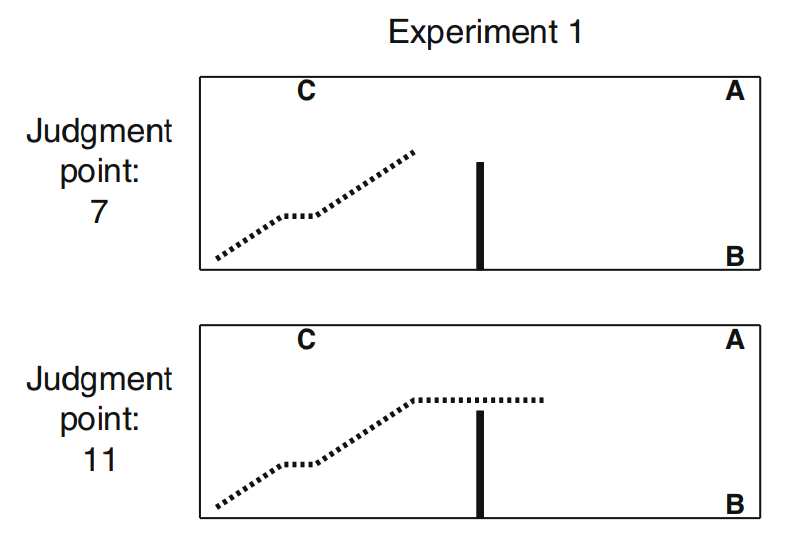
\includegraphics[width=0.7\linewidth, trim=15pt 0pt 0pt 15pt, clip]{intro/tenenbaum_exp}
	\caption{Example stimulus, from \citeA{baker2009}, Experiment 1. Participants watch a clip of what they are told is an agent moving in an environment. Three goals (A, B, C) are marked in the environment. The clip is stopped at various points in the trajectory (\textit{judgement points}), and the participants are asked to judge the probability of each goal being the goal pursued by the alien.}
	\label{fig:tenenbaum:env}
\end{figure}


The authors developed three models to solve the same task using inverse planning:
First, the environment is defined as a Markov Decision Problem for each of the goals, and the Boltzman policies are calculated. Then, with the given trajectory, the posteriors of the goals, given the trajectory, are determined. 
A more detailed account of the models will be given in \ref{subsec:models}. The authors also included a model based on a simple heuristic, as to which an agent's goal always corresponds to the one it has moved towards in the last step, thereby assessing the most likely goal continuously for each step, neglecting the history.

Lastly, the posterior goal likelihoods under each model are compared to the human participants' judgments. The authors found a good correlation between the models' predictions and the human judgments.

In this project, the modeling methods of \citeA{baker2009} will be used to create a framework with which agent movement in a 2D regular grid environment can be simulated, and, given real-life or simulated observations, inferences can be drawn to internal model parameters and structures using inverse planning.
Two types of representation are explored, the map-like regular grid representation used in \citeA{baker2009}, and a vector representation describing only distance and direction to the goals in the environment.
Moreover, the omniscient calculation process used in the original article is here contrasted with a greedy local algorithm for navigation. 

Most modeling approaches to insect navigation focus on simulating a specific skill observed in insects, such as the homing behavior in ants \cite<e.g.,>{goldschmidt2017a}, or the replication of behavior observed in specific neural circuits or areas.
Especially the insect central complex which has been connected to insect navigation \cite{honkanen2019}, is the subject of a variety of computational models \cite<e.g.,>{adden2020a,cope2017,stone2017}, which mostly focus on the topic of orientation and steering, but also on path integration.
A second neural structure that is a common target for computational modeling in the area of insect navigation is the mushroom body \cite<e.g.,>{ardin2016} to investigate insect memory.

These modeling approaches are mostly used to either replicate behavior found in in-vivo experiments, to answer questions about latent mechanisms by comparing viability of different computational approaches, or to generate new hypotheses.

This project focuses on a different question: it provides a framework for modeling approaches of trajectory-generating artificial agents.
These trajectories can then potentially be employed for the aforementioned usages of computational modeling by either asking theoretical questions, or by comparing it to real experimental data.
The inverse planning methods based on Bayesian inferences allows for freedom in the subject of researched questions and directionality and dependency of model variables.

This report is structured as follows: First, the basics of Markov Decision Problems will be explained. Second, the specific computations in the models from \citeA{baker2009} will be described.
Third, the implementation details and computations used in this project will be shown.
Fourth, three conducted experiments will be presented.
The report will be concluded with a discussion on possibilities of inverse planning for insect navigation research.

\iffalse
\section*{P1}

% P1
% all considered pathfinding algos
% evaluation

\subsection{Path-finding Algorithms}

\todo{Question: is random walk as efficient as exhaustive search if we do not know where the goal is?}

\begin{itemize}
	\item Random Walk
	\begin{itemize}
		\item Maximal Entropy Random Walk
		\item Correlated Random Walk
		\item Lévy Walk
	\end{itemize}
	\item Chemotaxis
	\item Greedy
	\item General and Exhaustive Search \cite{russell1995, deo1984, korf1988}
	\begin{itemize}
		\item MDP / Dijkstra
		\item Breadth-first search
		\item Uniform-cost search (Dijkstra \cite{dijkstra1959})
		\item Depth-first search
		\item Depth-limited
		\item Iterative deepening
		\item Bidirectional
		\item Bellman-Ford?
	\end{itemize}
	\item Informed Search
	\begin{itemize}
		\item Greedy Search -> always expand first the node that is deemed closest to the goal, based on a heuristic, e.g. straight-line distance; not guaranteed to find best path
		\item Best-First Search $\rightarrow$ GSM with informed queing/node expanding based on an evaluation function for the nodes \cite{russell1995}
		\item A* (Hart et al. 1968, 1972) (Dynamic weighting Pohl 1973?)
	\end{itemize}
	\item A* - deviants
	\begin{itemize}
		\item Heuristic Functions (Newell and Ernst, 1965) --> Iterative Deepening A*
		\item Hierarchical Path-Finding A* \cite{botea}
		\item SMA* (Simplified Memory-Bound A*)
		\item RBFS (Korf 1993), IE (Russell 1992); tabu search (Glover 1989); see Russell and Norvig p.116f
		\item Bidirectional A*
		\item Multi-Heuristic A* \cite{aine2016}
	\end{itemize}
	\item Biologically inspired
	\begin{itemize}
		\item *Beetle Antenna Search Algorithm* \cite{jiang2017}
	\end{itemize} 

\end{itemize}


\begin{itemize}
	\item Waypoint navigation
	\item Jump Point Search
	\item Wavefront Algorithm
	\item Simulated Annealing (typically combined with potential field method) \TODO{maybe integrate into greedy}
\end{itemize}
\fi

\section{Background}

% P2
% explain Tenenbaum
% explain MDP
% explain Tenenbaum Model
% Pathfinding algos adaptations to generate policies
% trajectory sampling
% results

\subsection{Markov Decision Problems}

The problem at hand is defined by \citeNP{baker2009} as a Markov Decision Problem (MDP; \citeNP{bellman1954}, \citeNP[p.~500 ff.]{russell1995}), even though the model itself has deterministic transitions instead of stochastic transitions which MDPs are usually used for. This has several advantages over classical path-finding algorithms in this scenario: First, it is possible to directly infer decision probabilities from the utility function, whereas classical path-finding algorithms usually provide action sequences, and probability functions would have to be calculated, leaving a large decision to the modeler. Second, it is possible to calculate a path to the goal from every state, therefore solving the Single-Destination Shortest Path problem. Third, it makes it possible to look at arbitrary partial trajectories without defining the end state of a particular trajectory as a goal, thereby allowing goal inferences for partial trajectories. Fourth, it is easy to change the model in the future, so for example to include stochastic transitions.

The main difference between classic path-finding problems and MDPs is that policies are calculated instead of action sequences, because action outcomes are stochastic.

In the following, the basics of MDPs will be defined after \citeNP[p.~500ff.]{russell1995}. 

\paragraph{Transition Model.}

A transition model describes the transition probabilities between states. $M^a_{ij}$ is the probability of reaching state $j$ from state $i$ by taking action $a$. Generally, \textit{Markov Property} holds, which means that transition probabilities are only dependent on the current state, and not on previous states in the history.

\paragraph{Policy.}
A policy $\pi$ is a mapping from a set of states $S$ to a set of actions $A$ \cite{russell1995} (p.500). Finding the optimal path translates to finding the optimal policy $\pi^*$, so choosing the optimal action for every state. This is done by assigning utilities to all states by determining the expected utility of being in a state $i$ and executing an optimal policy $\pi^*$.
This translates to the expected utility over all possible environment histories $H(i, \pi^*)$ generated by that policy after starting in state $i$:

\begin{equation}
	U(i) = EU(H(i, \pi^*)|M) = \sum P(H(i, \pi^*)|M)U_h(H(i,\pi^*))
\end{equation}

Here, $U_h$ denotes the utility functions on histories, and needs to be separable, meaning there exists a function $f$ such that $U_h([s_0, s_1,...,s_n]) = f(s_0, U_h(s_1, ..., s_n))$.
Taking rational then translates to choosing actions which promise the highest utility, according to the Maximum Expected Utility principle.

\paragraph{Markov Decision Problems.}

Markov Decision Problems are the problem of finding an optimal policy in a fully observable environment, whereby transitions in this environment are stochastic, but the transition model is known.


\paragraph{Value Iteration Algorithm.}\label{para:value_it}

To calculate an optimal policy, a \textit{dynamic programming} algorithm can be employed. One such algorithm is the \textit{Value Iteration algorithm}.

Let $R: S \rightarrow {\rm I\!R}$ be a \textit{reward function} that maps all states in the environment to a real value, for example based on move cost to this state, and whether the state is a goal or an obstacle.

Using the last definitions, and a utility function on histories which is additive, meaning $U_h([s_0, s_1,...,s_n]) = R(s_0) + U_h(s_1, ..., s_n)$. We can then equate the optimal policy $\pi^*$ of a state $i$ to 

\begin{equation}\label{eq:optimalpolicy}
	\pi^*(i) = \argmax_a \sum_{j} M_{ij}^aU(j)
\end{equation}
	

The utility of a state $U(i)$ can similarly be defined as 

\begin{equation}
U(i)  = R(i) + \max_a \sum_j   M_{ij}^aU(j)
\end{equation}

When applying this equation to all states repeatedly, the utilities eventually converge. From these utilities, the optimal policy can be chosen according to Equation \ref{eq:optimalpolicy}.

\subsection{Model Computations by \citeA{baker2009}}\label{subsec:models}

The models proposed by \citeA{baker2009} builds upon these classical calculations, however, some specifications are adapted. In the following part, the calculations by model M1 from \citeA{baker2009} will be outlined. All calculations are dependent on the given environment. However, since we assume the environment to be static, we will leave it out in the following definitions for the sake of simplicity.

\paragraph{Setup.}
The model is supplied with a set of states $S$ (i.e., the environment), a set of goals $G$, with $G \subseteq S$, a set of possible actions $A$, and a set of obstacles $O \subseteq S$ in the environment, with $O \cap  G = \emptyset$. Furthermore, a parameter $\beta$ is introduced, which specifies the determinism of the agent. With $\beta=0$, steps are taken randomly with no prioritization according to state utilities, with higher values of $\beta$, the agent moves increasingly deterministic.

From these context specifications, the transition matrix $T_{i,a,j}, i,j \in S, a \in A$ is inferred, which specifies all possible state transitions $i \overset{a}{\rightarrow} j$ in the environment. These can in theory be stochastic transitions, however, in this model, only deterministic transitions are considered. This means it is assumed that every action the agent takes has a deterministic outcome.
In this report, the transition model $T_{i,a,j}$ will be shortened to $T$. $T(i)$ then refers to all action-state pairs possible from state $i$. $T(i,a)$ denotes all states $j$ that can be reached from state $i$ with action $a$ (for generalizability; in the concrete calculations, this will always be a single state, as the transitions are deterministic).

\paragraph{Policy calculation.}
The next step is the calculation of the reward function $R: {S,A,S} \rightarrow  {\rm I\!R}$. This reward function is similar to the reward function specified in Section \ref{para:value_it}, but since the model accounts for diagonal movements, the move cost from an origin state $i$ is dependent on the destination state $j$. The reward function has to be specified for each goal $g \in G$.

\begin{equation}\label{eq:rewards}
	R(i,a,j | g)= 
	\begin{cases}
		\text{goal reward} + \text{move cost}(a),& \text{if } i = g\\
		\text{trap cost},              & \text{if } i \in O \\
		\text{move cost}(a) & \text{else}
	\end{cases}
\end{equation}%\[

%\]

Using these precalculations, a value iteration algorithm can be applied until a specified convergence tolerance is reached. The utility function is also calculated for every goal.

%\[
\begin{equation}
U_{t+1}(i|g) \leftarrow \underset{a}{\max} ( R(i,a,j|g) + \gamma U_t(j|g)  ), ~~~a,j \in T(i)
\end{equation}
%\]

$\gamma$ is a convergence factor specified by the modeler.

With the converged utility function, the policies can be determined. Contrary to classical policy calculations, the transitions themselves are not stochastic, but the decisions taken by the agent are.
This means that an agent does not always take the action which optimizes its utility, but takes actions stochastically, with the probabilities depending on the utilities. The optimal action is chosen with the highest probability, the second best with the second highest probability and so on.

This is done by taking the soft-max of the utilities multiplied with the determinism factor $\beta$:

Let $\pi$ be a policy, then the probability of taking action $a$ in state $i$, given that the agent pursues  goal $g$ is

%\[
\begin{equation}\label{eq:boltzmann}
P_\pi(a|i,g) = \frac{exp(  \beta(  R(i,a,j|g) + \gamma U(j|g)  )  )}{ \sum_{T_i}  exp(  \beta(  R(i,a,j|g) + \gamma U(j|g)  )  )}
\end{equation}
%\]
for all $a,j \in T(i)$.

\paragraph{Goal inference.}
The last step in the model is the inversion of the planning algorithm applied before. 
Given a trajectory up to a time point $T$, $\{ s_0, s_1, ..., s_T  \}$ with $s_0,...,s_n \in S$, the posterior probabilities $P(G=g|s_0,...,s_T)$ are calculated for every goal.

This is done by recursively calculating the likelihoods of the partial trajectories in $t$, given the priors over the goals $P(G)$. In each step, $a$ denotes all possible actions that can lead from a state $s_t$ to the next state $s_{t+1}$ in the trajectory.


\begin{flalign*}
		& P(s_0|G=g) = P(g) \\
		& P(s_0, s_1 | G=g) = P(s_0 | G=g) \cdot P_\pi(a | s_0, g) \\
		& ... \\
		& P(s_0, ...,s_T | G=g) = P(s_0,...,s_{T-1} | G=g) \cdot P_\pi(a | s_{T-1}, g)
\end{flalign*}

Using Bayes' Rule, these likelihoods can be inverted, which predicts, which of the goals in the environment is most likely the pursued goal, given the observed trajectory:

\begin{equation}\label{eq:posteriors}
	P(g|s_1,...,s_T) \propto P(s_2,...,s_T|s_1, g) \cdot P(g)
\end{equation} 

\input{intro/trajectory_sampling.tex}

\section{Method}

As a basis for this project, the implementation of inverse planning on \url{https://github.com/stacyste/TheoryOfMindInferenceModels} was used.
The implementation was done in Python 3, and kept in the same language for this project. However, additions to the language from Python 3.9 are used.
To allow for expansion and the implementation of different methods, the code base was made modular.
Another method of representing states, and another way of navigating was implemented.
Furthermore, the implementation was sped up.
Moreover, a testing environment was created to ensure functionality of the original example scenarios and all expansions.
In the following, the main modules, its functionality, and usage will be explained.

\subsection{Dependencies}
The program has the following dependencies:
\begin{itemize}
	\setlength\itemsep{0em}
	\item numpy\footnote{numpy.org/}
	\item pandas\footnote{pandas.pydata.org/}
	\item matplotlib\footnote{matplotlib.org/}
	\item tqdm\footnote{tqdm.github.io/}
\end{itemize}

\subsection{Representation Types}
\subsubsection{Map-like Regular Grid Representation}
To represent the environment, the modeling approach in \citeA{baker2009} uses a regular grid map-like representation with 2D squares discretizing the environment.
This is a popular choice for navigation models (cf. e.g., \citeNP{algfoor2015}).

\subsubsection{Vector-based Representation}
The other representation type that was implemented in this project is a vector representation of the goals.
The states in the environment are discretized just like in the map-like representation. However, the agent has no access to the cell in the grid itself, and its position.
To the agent, the cell is a set of vectors that describe the distance and the direction to all goals in the environment.


\subsection{Loading Experimental Data}
A new module was created to allow the loading of experimental data into the program.
A full example of this can be found in the appendix in Section \ref{appendix:ex_loading}.

The module is developed to load data of the following form:
First, the configuration is specified using YAML \footnote{\url{yaml.org/}}.
In this configuration, the shape of the arena needs to be specified. Currently, two shapes are possible: circles and rectangles.

A circular arena is configured as follows.

\begin{verbatim}
	#     Circle:
	#       center_x: 4
	#       center_y: 4
	#       radius: 3
\end{verbatim}

The discrete cells which are included in the circular arena are calculated quadrant-wise. Around the center of the circle ($centerX, centerY$), all cells are included for which

\[
(x - centerX)^2 + (y - centerY)^2 < r
\]

\noindent
holds for the inner corner of the cell.

The center of the circle is transformed to $(0,0)$, so the discretization is independent of the center. This issue can be demonstrated with a simple example, as shown in Figure \ref{fig:circle_issue}. The resulting arena of the example configuration can be seen in Figure \ref{fig:circular_arena}.

\begin{figure}[htb]
	\centering
	\resizebox{0.95\linewidth}{!}{%
		\subcaptionbox{{\large Circle with center $(2,2)$ and radius $1.5$.}}{
			\begin{tikzpicture}
				\tkzInit[xmax=4,ymax=4,xmin=0,ymin=0]
				\begin{scope}[dotted]
					\tkzGrid[color=black!50, line width = 0.3pt]
				\end{scope}
				%\tkzGrid
				%\draw[ thick,latex-latex] (-1,4) -- (4,-6) node[anchor=south west] {$a$}; % two points for drawing 2x+y=2
				\foreach \x/\y in {1/1, 1/2, 1/3, 1/4, 2/1, 2/2, 2/3, 2/4, 3/1, 3/2, 3/3, 3/4, 4/1, 4/2, 4/3, 4/4}
				\filldraw[draw=CornflowerBlue,fill=CornflowerBlue!10, fill opacity=1] (\x-1,\y-1) rectangle (\x, \y);
				\filldraw[draw=red,fill=red!20, fill opacity=.4] (2,2) circle (1.5);
				\tkzAxeXY
			\end{tikzpicture}
		}%
		%\hfill
		\hspace{0.1\linewidth}
		\subcaptionbox{{\large Circle with center $(1.5,1.5)$ and radius $1.5$.}}{
			\begin{tikzpicture}
				\tkzInit[xmax=4,ymax=4,xmin=0,ymin=0]
				\begin{scope}[dotted]
					\tkzGrid[color=black!50, line width = 0.3pt]
				\end{scope}
				%\tkzGrid
				
				%\draw[ thick,latex-latex] (-1,4) -- (4,-6) node[anchor=south west] {$a$}; % two points for drawing 2x+y=2
				\foreach \x/\y in {1/1, 1/2, 1/3, 2/1, 2/2, 2/3, 3/1, 3/2, 3/3}
				\filldraw[draw=CornflowerBlue,fill=CornflowerBlue!10, fill opacity=1] (\x-1,\y-1) rectangle (\x, \y);
				\filldraw[draw=red,fill=red!20, fill opacity=.4] (1.5,1.5) circle (1.5);
				\tkzAxeXY
			\end{tikzpicture}
		}%
	}
	\caption{Discretization of circles can differ depending on the center.}
	\label{fig:circle_issue}
\end{figure}

\begin{figure}[htb]
	\begin{center}
		\resizebox{0.75\linewidth}{!}{%
			\begin{tikzpicture}
				\tkzInit[xmax=7,ymax=7,xmin=0,ymin=0]
				\begin{scope}[dotted]
					\tkzGrid[color=black!50, line width = 0.3pt]
				\end{scope}
				%\tkzGrid
				
				%\draw[ thick,latex-latex] (-1,4) -- (4,-6) node[anchor=south west] {$a$}; % two points for drawing 2x+y=2
				\foreach \x/\y in {1/3, 2/3, 1/6, 3/2, 2/6, 4/3, 3/5, 5/3, 4/6,
					6/2, 5/6, 6/5, 1/1, 2/1, 1/4, 3/6, 2/4, 4/1,
					3/3, 6/3, 5/1, 4/4, 6/6, 5/4, 4/2, 3/1, 1/2,
					3/4, 2/2, 1/5, 4/5, 6/1, 2/5, 5/5, 6/4, 5/2}
				\filldraw[draw=CornflowerBlue,fill=CornflowerBlue!10, fill opacity=1] (\x-1,\y-1) rectangle (\x, \y);
				\filldraw[draw=red,fill=red!20, fill opacity=.4] (3,3) circle (3);
				\tkzAxeXY
			\end{tikzpicture}
		}
	\end{center}
	\caption{Circular arena with a center at $(3, 3)$ and a radius of $3$. The center was transformed from the original $(4,4)$. The circle is approximated by including all discrete cells with at least one corner within the specified circle.}
	\label{fig:circular_arena}
\end{figure}

A rectangular arena is specified similarly:

\begin{verbatim}
	#     Rectangle:
	#       center_x: 4
	#       center_y: 4
	#       grid_width: 6
	#       grid_height: 6
\end{verbatim}

The center is transformed to $(grid\_width/2,grid_height/2)$, such that the lower left corner adheres to $(0,0)$. This gives an arena as expected, which is depicted in Figure \ref{fig:rect_arena}.

For both shapes, all specifications have to be $\geq$ 0.

\begin{figure}[htb]
	\centering
	\resizebox{0.75\linewidth}{!}{%
	\begin{tikzpicture}
		\tkzInit[xmax=7,ymax=7,xmin=0,ymin=0]
		\begin{scope}[dotted]
			\tkzGrid[color=black!50, line width = 0.3pt]
		\end{scope}
		
		\foreach \x in {1,...,6}
			\foreach \y in {1,...,6}
				\filldraw[draw=CornflowerBlue,fill=CornflowerBlue!10] (\x-1,\y-1) rectangle (\x,\y);
		\tkzAxeXY
	\end{tikzpicture}
	}
	\caption{Rectangular arena created with the specifications of a center at $(0,0)$, transformed from $(4,4)$, a height of $6$ and a width of $6$.}
	\label{fig:rect_arena}
\end{figure}



After the YAML specification, the data file must contain position data from a single agent in a single trial.
This data is discretized to match the grid specified before.

The module \module{io} implements a reader class \module{CSVReader}, illustrated in Figure \ref{fig:uml:csvreader}, which provides the means to load this type of data.
The arena dimensions specified in the data file can be accessed via the \module{dimensions} function provided by the \module{CSVReader}. Currently this module can load arenas of circular and rectangular shapes.
The positional recordings can be accessed using the \module{trajectory} function.

\definecolor{classcolor}{HTML}{F3B3A9}
\tikzumlset{fill class=classcolor!30}
\begin{figure}
	\centering
\begin{tikzpicture}
		\umlclass[ ] {io::CSVReader}{
			data\_path : str \\ pixelation : int
		}{read() : pandas.DataFrame \\ raw\_data() : pandas.DataFrame \\ read\_partial(requirements) : pandas.DataFrame \\ dimensions() : dict \\ trajectory(pandas.DataFrame) : list}
\end{tikzpicture}
\caption{Class \module{CSVReader} is used to load trajectory data into the program, and parse settings from the file, such as the dimensions of the arena.}
\label{fig:uml:csvreader}
\end{figure}

Sometimes, e.g. due to performance requirements, it might be desired to increase the rasterization of the environment to reduce the overall number of cells in the grid.
This can be done using the optional initiation parameter \module{pixelation} for the \module{CSVReader} class (see Figure \ref{fig:uml:csvreader}).
By default, this parameter is set to $1$, meaning no downsampling of states is undertaken.
Higher values will result in a smaller problem space.

From the parsed environment dimensions, an \module{Environment} object can be created (see Figure \ref{fig:uml:environment}).
In this step, goals and obstacle positions need to be provided, with their positions adjusted to the in the loading step specified pixelation.
An example environment can be seen in Figure \ref{subfig:env}.
Goals should be specified as a \module{Goal} object, see Figure \ref{fig:uml:goal}.
These specifications are then combined to an \module{MDP} object (see Figure \ref{fig:uml:mdp}), which provides the methods to describe the problem as a Markov Decision Problem.

\begin{figure}
	\centering
		\begin{tikzpicture}
		\umlclass[ ] {model::Goal}{
			name : str \\ pos : tuple[int, int] \\ reward : float
		}{}
	\end{tikzpicture}
	\caption{Class \module{Goal} is used to represent a goal in the environment, with respective position and reward, as well as a name for readability.}
	\label{fig:uml:goal}
	\begin{tikzpicture}
		\umlclass[] {model::Environment}{
			goals : [Goal] \\ obstacles : [tuple[int, int]] \\
			coords : [tuple[int, int]]
		}{}
	\end{tikzpicture}
	\caption{Class \module{Environment} represents an experimental environment, including goals and obstacles.}
	\label{fig:uml:environment}
	
	\begin{tikzpicture}
	\umlclass[] {model::MDP}{
		environment : Environment \\
		T : all possible transitions in environment
	}{reward\_table() : mapping from T to rewards}
	\end{tikzpicture}
	\caption{Class \module{MDP} represents the theoretical foundations for solving an MDP.}
	\label{fig:uml:mdp}
\end{figure}

To make these steps easier, a specific type of model is provided which executes these steps autonomously.
The \module{DataModel} class, provided by the \module{Model} module, implements the loading and adjusting procedures.

\subsection{Data Sampling}

The second possibility is to sample a trajectory instead of loading it from data.
This is done via the \module{SamplingModel} class.
An example can be found in the appendix, Section  \ref{appendix:ex_sampling}.
The arena dimensions can be either loaded from a file with specified configurations, or defined manually.
No transformation is taking place, so the center needs to be defined as $(width/2, height/2)$, or $(radius, radius)$ for a circular arena.
Goals and obstacles have to be specified as described in the previous section on how to load experimental data.

Another required parameter is the starting position, which can be any position in the specified environment, and which can also be specified in a configuration file.

The class implements a method to sample a goal according to either specified goal priors, or a uniform distribution.
With a chosen goal, which can also be chosen manually be the modeler, the class can then sample trajectories using the method \module{sample\_trajectory}.
This is done using a policy over the environment.
This policy has to be calculated, which will be explained in the following.

\iffalse
\begin{figure}
	\begin{tikzpicture}
		\umlclass[ ] {model::SamplingModel}{
			dimensions : dict \\ goals : list \\ obstacles : list \\ start\_pos : 
		}{\_\_init\_\_(dimensions : dict, goals : list, obstacles : list, start\_pos : tuple[int, int])}
	\end{tikzpicture}
	\caption{\TODO{description} \TODO{simplified}, e.g. no agent class}
	\label{fig:uml:samplingmodel}
\end{figure}
\fi

\subsection{Policy Calculation}
Before policies can be calculated, the previously specified models are used to generate \module{MDP} objects, which provide methods that grant easy access to constructs used by MDP solving algorithms, such as the reward function, or the transition model.

Policies are calculated internally in the \module{Model} class and all its children using implementations of the \module{Solver} class, provided by the \module{calcs.mdp} package. 
The \module{Solver} class provides the function \module{calculate\_policies(goal : Goal, beta : float)}, which has to be implemented by inheriting classes, and calculates policies to a given goal, using the determinism factor beta ($\beta$ in Equation \ref{eq:boltzmann}).
Currently, two implementations exist: the \module{OptimalSolver} class (see Figure \ref{fig:uml:optimalsolver}), which implements the value iteration algorithm employed by \citeA{baker2009}, and the \module{GreedySolver}.
Utility values of the in an exemplary environment can be seen in Figure \ref{fig:utilities}. 

\paragraph{Optimal Solver.}

\begin{figure}
	\centering
	\begin{tikzpicture}
		\umlclass[ ] {calcs.mdp::OptimalSolver}{
			mdp : MDP \\ beta : float \\ utilities : dict \\ gamma : float \\ reward\_table : dict
		}{+\_\_init\_\_(mdp : MDP, gamma : float =.95) \\ +policies(goal : Goal) \\ -\_q\_value(state : State, action : tuple[int, int], goal : Goal) : float \\ -\_value\_iteration(goal : Goal) : dict \\ -\_get\_boltzmann\_policy(state: State, goal : Goal) : dict}
	\end{tikzpicture}
	\caption{The class \module{OptimalSolver} takes a description of a Markov Decision Problem (in the form of an \module{MDP} object), and solves it via value iteration.}
	\label{fig:uml:optimalsolver}
\end{figure}

A class diagram of the \module{OptimalSolver} can be seen in Figure \ref{fig:uml:optimalsolver}.
This module implements the method used in \citeA{baker2009}.
Calling the function \module{policies(goal)} internally calls the \module{\_value\_iteration} function.
This algorithm as applied to one goal in the environment, with a reward table specific to that goal, is illustrated in the following:

\begin{algorithm}
	\SetAlgoLined
	\DontPrintSemicolon
	\KwResult{Utility function $U: S \rightarrow {\rm I\!R}$}
	\SetKwInOut{Input}{input}\SetKwInOut{Output}{output}
	\SetKwFunction{QValue}{\_q\_value}
	\SetKwProg{Fn}{def}{:}{}
	\Input{convergence tolerance $\epsilon$, all states $S$ in MDP, transition model $T$, reward function $R$, discount factor $\gamma$ (default $=.95$)}
	\BlankLine
	$\Delta \leftarrow$  $\epsilon \cdot$ 100\;
	$U(i) \leftarrow$ 0 for all $i \in S$\;
	\While{$\Delta > \epsilon$}{
		$\Delta \leftarrow 0$\;
		\For{$i \in S$}{
		$U_{t+1}(i) \leftarrow max($\QValue{$i, a, \gamma $}$)$ for all $a \in T(i)$\;
		$\Delta \leftarrow max(\Delta, | U_t(i) - U_{t+1}(i) |)$
		}
	}
	\BlankLine
	\Fn{\QValue{i, a, $\gamma$}}{
		\KwRet{$\sum_{j \in T(i,a)} R(i,a,j) +  \gamma \cdot U_t(j)$}
	}
	\caption{Value Iteration}
\end{algorithm}

Finally, the soft-max/Boltzmann policy is calculated according to Equation \ref{eq:boltzmann}.
If any of the values $\beta(  R(i,a,j|g) + \gamma U(j|g))$ exceeds $700$, all values are scaled to the range $(0,700)$ to prevent overflow.



\paragraph{Greedy Solver.}
The greedy variant of policy generation for a specific goal $g$ is calculated as follows:
First, the reward table $R(i,a,j)$ from Eqn. \ref{eq:rewards} is updated with the reward of the goal $g$:

\[
R(i,a,j) = \begin{cases}
	R(i,a,j) + goal~reward(g) & \text{if j = g}\\
	R(i,a,j) & \text{else}
\end{cases}
\]

The policy is then calculated according to the following algorithm:

\begin{algorithm}
	\SetAlgoLined
	\DontPrintSemicolon
	\KwResult{Utility function $U: S \rightarrow {\rm I\!R}$}
	\SetKwInOut{Input}{input}\SetKwInOut{Output}{output}
	\SetKwFunction{QValue}{\_q\_value}
	\SetKwFunction{Dist}{distance\_to\_goal}
	\SetKwData{MaxDist}{max\_dist}
	\SetKwProg{Fn}{def}{:}{}
	\Input{all states $S$ in MDP, transition model $T$, reward function $R$, discount factor $\gamma$ (default $=.95$)}
	\BlankLine
	\For{transitions $(i,a,j) \in T$}{
		\If{j = g}{
			$R(i,a,j) \leftarrow R(i,a,j) + goal~reward(g)$
		}
	}
	\MaxDist$\leftarrow max(\Dist{k,g}) \text{ for all } k\in S$\;
	$U(i) \leftarrow \MaxDist - \Dist{i,g} $\; % {state: (max_distance - state.distance[goal.name]) for state in self.mdp.agent_states}
	\caption{Greedy Utility Calculation}
\end{algorithm}

The soft-max/Boltzmann policy is then calculated as in the Optimal Solver illustrated before.


\subsection{Goal Inference}

After a trajectory is either observed or sampled from a model, the posterior likelihoods of all goals in the environment can be inferred as described in Equation \ref{eq:posteriors}.
An example of this can be seen in Figure \ref{fig:posteriors}.

\begin{algorithm}
	\SetAlgoLined
	\DontPrintSemicolon
	\KwResult{Goal likelihoods in every time step}
	\SetKwInOut{Input}{input}\SetKwInOut{Output}{output}
	\SetKwFunction{QValue}{\_q\_value}
	\SetKwFunction{ProbNext}{$P_\pi$}
	\SetKwProg{Fn}{def}{:}{}
	\Input{all states $S$ in MDP, goal priors $P(G)$, goals $G$, trajectory $\{s_0, ..., s_T\}$, Goal-dependent policies \ProbNext}
	\BlankLine
	
	$P(s_0|g)\leftarrow P(g)$\;% p_state_t_neg_log = np.log(np.array([priors] * len(trajectory)))
	\For{time step $t$ in trajectory}%	    for time, state in enumerate(trajectory[:-1]):
	{
		\For{goal $g$ in $G$}{
			$P(s_0,..,s_{t+1}|g) = P(s_0,..,s_t|g) $\\ \Indp$ \cdot $\ProbNext$(s_t \rightarrow s_{t+1} | s_t, g )$
		}
	}
	
	\For{time step $t$ in trajectory}{
		$P(s_0,..,s_t | g) = P(s_0,..,s_t | g) \cdot P(g)$\;
		$P(s_0,..,s_t | g) = P(s_0,..,s_t | g) / \sum_{h \in G} P(s_0,..,s_t | h)  $
	}
	\caption{Calculation of Goal Likelihoods}
\end{algorithm}

This algorithm gives the likelihood of all goals for each time step in the trajectory.

\begin{figure}
	\centering
	%\resizebox{0.95\linewidth}{!}{%
	\subcaptionbox{{\normalsize Example environment with two states, A and B, and two obstacle states in the middle.}\label{subfig:env}}{
	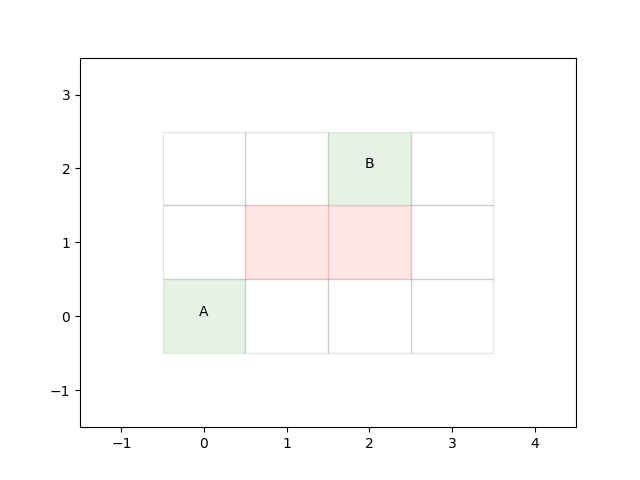
\includegraphics[width=.95\linewidth, clip, trim=3cm 3cm 3cm 3cm]{res/env}
	}
	\subcaptionbox{{\normalsize Utility values for the goal in the upper right (dark green), produced by the \module{OptimalSolver} class.}\label{subfig:utilities_optimal}}{
	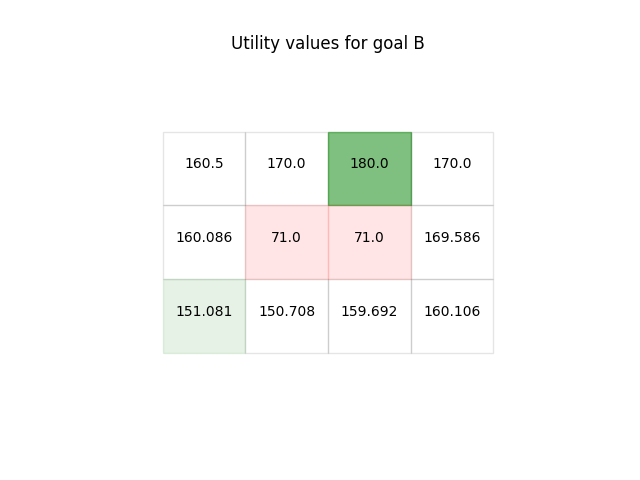
\includegraphics[width=.95\linewidth, trim=3cm 3cm 3cm 2cm,clip]{res/utilities_optimal}
	}
	\subcaptionbox{{\normalsize Utility values for the goal in the upper right (dark green), produced by the \module{GreedySolver} class.}\label{subfig:utilities_greedy}}{
		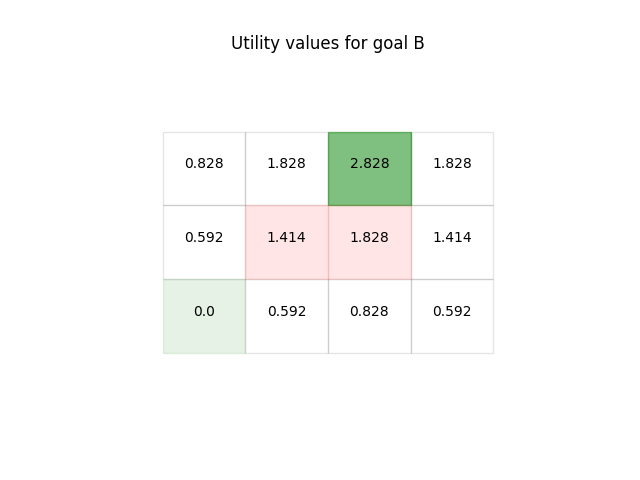
\includegraphics[width=.95\linewidth, trim=3cm 3cm 3cm 2cm,clip]{res/utilities_greedy}
	}
	%}
	\caption{Utilities for the two navigation methods applied to the environment in (a). Note that the greedy method assigns relatively high values for the two obstacle states, as they are right next to the goal state; if the actions towards obstacles are taken by the agent, it effectively stays on the state it was in.}
	\label{fig:utilities}
\end{figure}

\begin{figure}
	\centering
	\subcaptionbox{{\normalsize A trajectory to goal B in the upper right, starting from the lower right corner. The numbers indicate the time step.}\label{subfig:trajectory}}{
	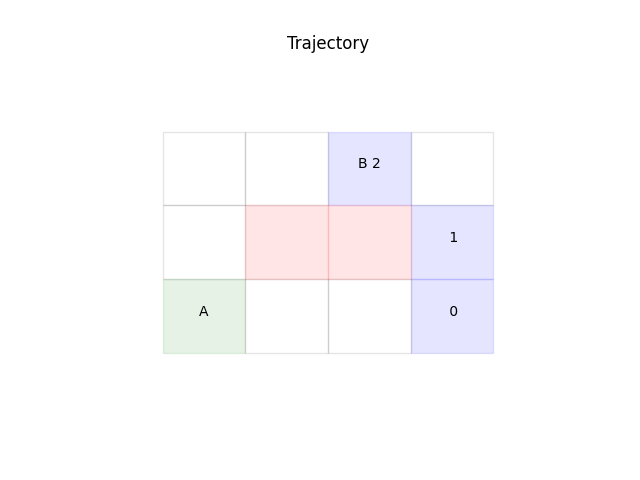
\includegraphics[width=0.95\linewidth, clip, trim=3cm 3cm 3cm 3cm]{res/trajectory}
	}
	\subcaptionbox{{\normalsize Posterior probabilities of the goals A and B, according to the optimal policies produced by the \module{OptimalSolver} class.}\label{subfig:posteriors_optimal}}{
	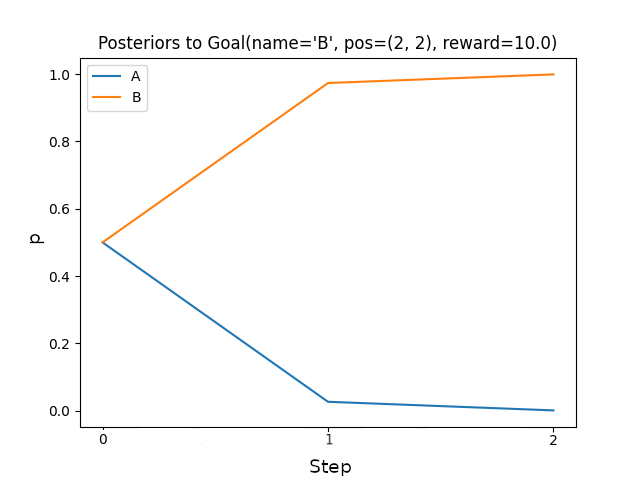
\includegraphics[width=0.95\linewidth]{res/optimal_pos}
	}
	\subcaptionbox{{\normalsize Posterior probabilities of the goals A and B, according to the optimal policies produced by the \module{GreedySolver} class.}\label{subfig:posteriors_greedy}}{
	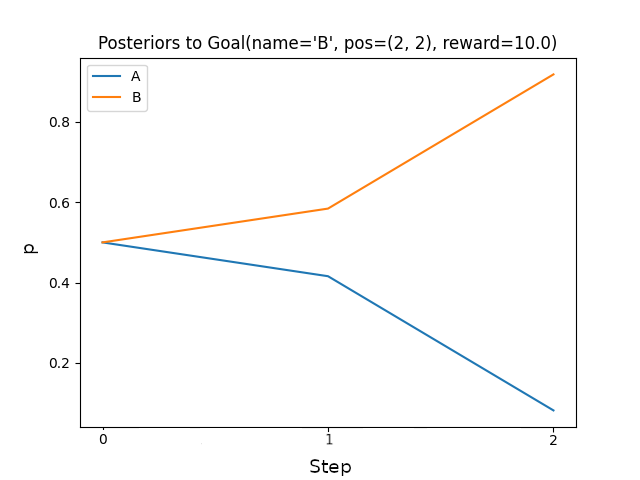
\includegraphics[width=0.95\linewidth]{res/greedy_pos}
	}
	\caption{Posterior goal probabilities of goals A and B, after applying inverse planning with both navigation methods to the trajectory in (a).}
	\label{fig:posteriors}
\end{figure}


\subsection{Model Likelihood}

The likelihood of different models can be calculated analogous to goal likelihood given an observed trajectory.
For a trajectory $\{s_0,..,s_T\}$, the likelihood of a model $M$ can be established via Bayes' Rule:

\begin{equation}
	P(M | \{s_0, ..., s_T\}) \propto P(\{s_0, ..., s_T\} | M) \cdot P(M)
\end{equation}

In practice, the algorithm differs slightly from the algorithm for goal likelihood calculation.
The models have to be processed sequentially, since the states in the trajectory are model-dependent. States in the environment, i.e., positions or cells in the grid, are transformed into the representation used by the specific models.
This means that internally, the trajectories are represented differently.
The results of each evaluated model are later concatenated and treated as in the calculation of goal likelihoods.


\subsection{Experiments}
To show the viability of the framework, three experiments were conducted and the a fixed set of models was tested in these three conditions.
The evaluated models were all combinations of the two representation type (``GridState" and ``VectorState"), the two navigation types (``Optimal" and ``Greedy") and different values of the determinism parameter $\beta$.
Considered values were:

\[
[0,.5,1,2,3,5]
\]

In total, this amounted to 24 model variants.
Both experiments were conducted in a rectangular arena with the dimensions $\{width=20, height=20\}$.
Per experiment, 100 iterations were run, with the true model being chosen randomly from the aforementioned 24 model variants.

\subsubsection{Experiment 1}
For the first experiment, goals and starting point were chosen at random. The only limitation was that the starting point could not be set to the position of any of the goals.
No obstacles were placed in the environment.

\subsubsection{Experiment 2}
For the second experiments, starting position and goals were fixed.
The starting position was always set to the lower left corner $(0,0)$. Goals were placed on symmetric positions in the upper right quarter of the environment.
Goal placement can be seen in Figures \ref{fig:exp2convexobstacles} and Figure \ref{fig:exp2concaveobstacles}.
Two types of obstacles were placed in the environment: convex, and concave.

\paragraph{a) Convex Obstacles}
The convex obstacle can be seen in Figure \ref{fig:exp2convexobstacles}.
Convex obstacles in general are easier to navigate since usually the utility gradient naturally leads around the obstacle.

\begin{figure}
	\centering
	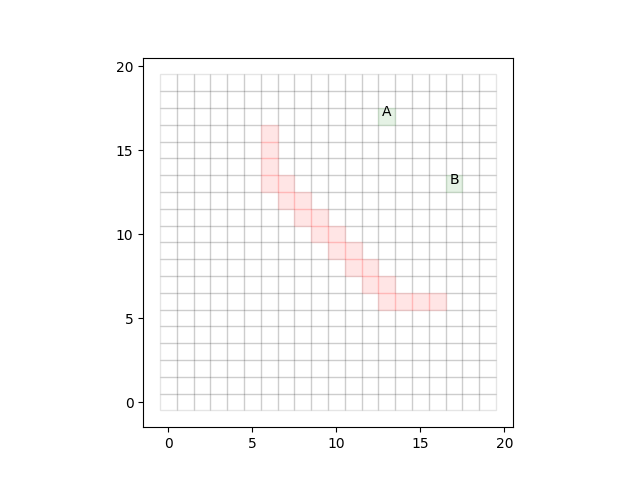
\includegraphics[width=0.8\linewidth]{res/exp2_convex_obstacles}
	\caption{Visualization of Experiment 2a with a convex obstacle between start and goals. Starting position, not depicted in this image, is the lower left corner. Two goals exist in the environment, Goal A and Goal B, whereas Goal A is the true goal and Goal B is the distractor.}
	\label{fig:exp2convexobstacles}
\end{figure}


\paragraph{b) Concave Obstacles.}
The concave obstacle can be seen in Figure \ref{fig:exp2concaveobstacles}.
Concave obstacles present a problem for traditional greedy forms of navigation,
as they introduce a local minimum.
As there were no specific methods implemented to avoid the agent getting caught in local minima, except for the determinism factor, the algorithm was set to end at a maximum of 3000 steps if the goal was not reached.


\begin{figure}
	\centering
	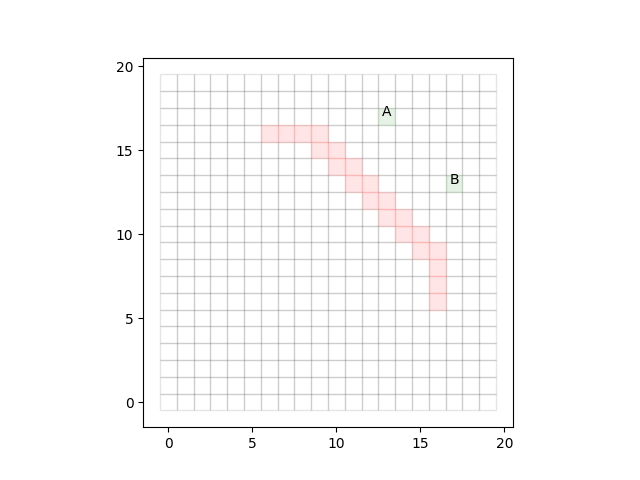
\includegraphics[width=0.8\linewidth]{res/exp2_concave_obstacles}
	\caption{Visualization of Experiment 2b with a concave obstacle between start and goals. Starting position, not depicted in this image, is the lower left corner. Two goals exist in the environment, Goal A and Goal B, whereas Goal A is the true goal and Goal B is the distractor.}
	\label{fig:exp2concaveobstacles}
\end{figure}



\section{Results}

In general, representation types could not be distinguished, meaning model variants of the same specification regarding $\beta$ parameter and algorithm type but with differing representation types were of the same likelihood.
Therefore, representation types will be ignored in the following section, and model likelihoods are capped at $50\%$, because there will always be a tie with the model variant with the other representation type.

\subsection{Experiment 1}
\begin{figure}
	\centering
	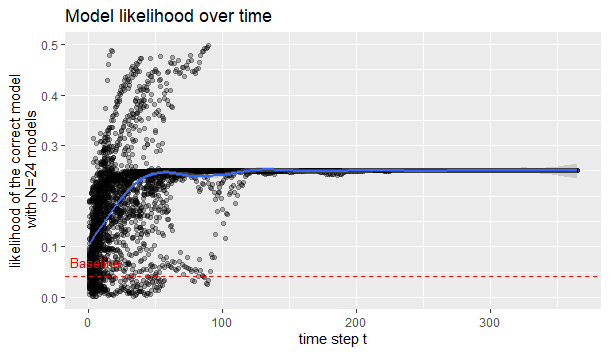
\includegraphics[width=0.95\linewidth]{../../statistics/R_noobst_t_likelihoodall}
	\caption{Likelihood of the true model over the time steps of the trajectories for Experiment 1 with no obstacles and randomized start and goal positions. The p values are drawn in black, whereas the blue line shows the generalized additive model.}
	\label{fig:rnoobsttlikelihoodall}
\end{figure}

Over all 100 trials, the mean length of the trajectories was 62.2 steps (median=13, SD=112.93), with a minimum of 1 step and a maximum of 365 steps.
For models with greedy algorithm type, the mean number of steps was 72.61, whereas for optimal algorithm type, the mean number was 49.98.

Evolution of likelihood for the true, generating model (i.e. the ground truth), over time can be seen in Figure \ref{fig:rnoobsttlikelihoodall}. At the last step of each trajectory, mean likelihood of the true model was .178 (median=.158, SD=.124).

\begin{figure}
	\centering
	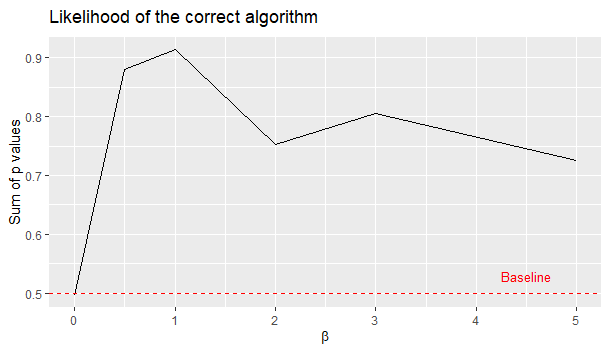
\includegraphics[width=0.95\linewidth]{../../statistics/R_noobst_beta_likelihoodalgo}
	\caption{Likelihood of the correct algorithm in Experiment 1 for all levels of $\beta$, calculated by summing up the p values of all models with the same algorithm as the true model.}
	\label{fig:rnoobstbetalikelihoodalgo}
\end{figure}

The true model is in most cases among the models with the highest likelihood, on average, around 87\% of model variants were worse than the true model (SD= .19).
On average, in 48\% of trials, the true model is among the models with the highest likelihood.
In these cases, all other models with the same likelihood share the same $\beta$ (determinism) factor, but employ the other representation and algorithm types.


Algorithm type could be distinguished, with a certainty of at least $95\%$, in $45\%$ of trials.
A distribution over the different levels for $\beta$ and the respective likelihood of the correct algorithm can be found in Figure \ref{fig:rnoobstbetalikelihoodalgo}.

\begin{figure}
	\centering
	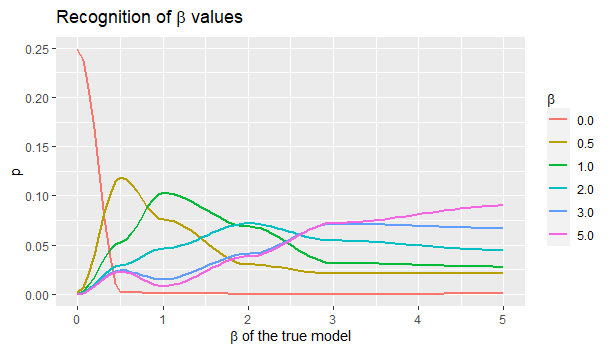
\includegraphics[width=0.95\linewidth]{../../statistics/R_noobst_beta_beta}
	\caption{Summarized p values of all model variants with the specific levels of $\beta$ values for Experiment 1. X axis shows the $\beta$ levels of the true model, colored lines show the local polynomial regression fit of the respective summarized p values of the model variants with specific $\beta$ values.}
	\label{fig:rnoobstbetabeta}
\end{figure}

Likelihoods of the different $\beta$ values relative to the $\beta$ value of the true model can be seen in Figure \ref{fig:rnoobstbetabeta}.



\subsection{Experiment 2}
\subsubsection*{a) Convex Obstacles}

Mean length of the trajectories was 316.6 steps (median=130.5, SD=455.07), with a minimum of 24 steps and a maximum of 2547 steps.
For models with greedy algorithm type, the mean number of steps was 571.4, whereas for optimal algorithm type, the mean number was 81.35.

Evolution of likelihood for the true, generating model, over time can be seen in Figure \ref{fig:rconvextlikelihoodall}. At the last step of each trajectory, mean likelihood of the true model was .365 (median=.434, SD=.145).

The true model is in most cases among the models with the highest likelihood, on average, around 98.7\% of model variants were worse than the true model (SD= .041).
On average, in 89\% of trials, the true model is among the models with the highest likelihood.
In these cases, all other models with the same likelihood share the same $\beta$ (determinism) factor, but employ the other representation type as discussed before.


Algorithm type could be distinguished, with a certainty of at least $95\%$, in $87\%$ of trials.
A distribution over the different levels for $\beta$ and the respective likelihood of the correct algorithm can be found in Figure \ref{fig:rconvexbetaalgosum}.


\begin{figure}
	\centering
	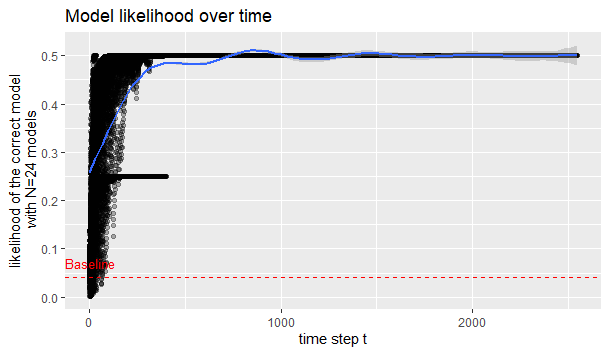
\includegraphics[width=0.95\linewidth]{../../statistics/R_convex_t_likelihoodall_points}
	\caption{Likelihood of the true model over the time steps of the trajectories for Experiment 2a with convex obstacles. The p values are drawn in black, whereas the blue line shows the generalized additive model.}
	\label{fig:rconvextlikelihoodall}
\end{figure}

\begin{figure}
	\centering
	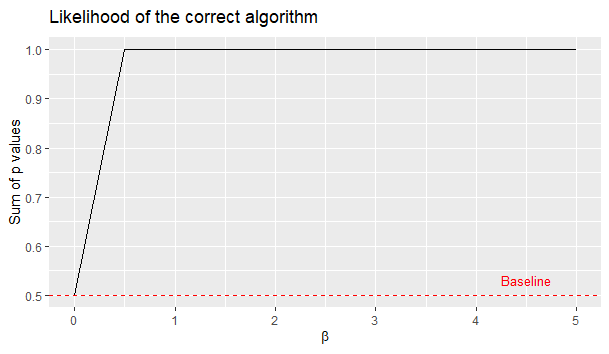
\includegraphics[width=0.95\linewidth]{../../statistics/R_convex_beta_algosum}
	\caption{Likelihood of the correct algorithm in Experiment 2a for all levels of $\beta$, calculated by summing up the p values of all models with the same algorithm as the true model.}
	\label{fig:rconvexbetaalgosum}
\end{figure}

\begin{figure}
	\centering
	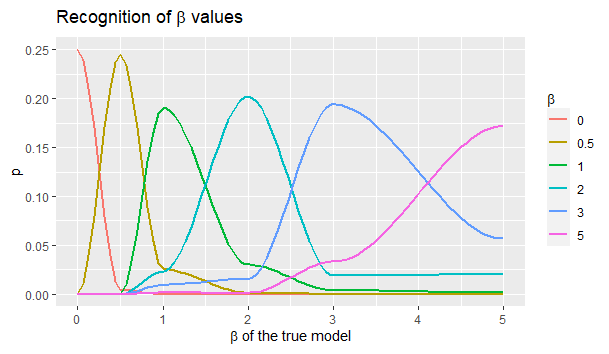
\includegraphics[width=0.95\linewidth]{../../statistics/R_beta}
	\caption{Summarized p values of all model variants with the specific levels of $\beta$ values for Experiment 2a. X axis shows the $\beta$ levels of the true model, colored lines show the local polynomial regression fit of the respective summarized p values of the model variants with specific $\beta$ values.}
	\label{fig:rbetaconvex}
\end{figure}

Likelihoods of the different $\beta$ values relative to the $\beta$ value of the true model can be seen in Figure \ref{fig:rbetaconvex}.

\subsubsection*{b) Concave Obstacles}

During the trials, between 24 and 2460 time steps were taken, with a mean of 499.5 (median=396, SD=536.26).
For models with greedy algorithm type, the mean number of steps was 531, whereas for optimal algorithm type, the mean number was 70.92.

Evolution of likelihood for the true, generating model, over time can be seen in Figure \ref{fig:rtlikelihoodall}. At the last step of each trajectory, mean likelihood of the true model was .388 (median=.5, SD=.144).

The true model is in most cases among the models with the highest likelihood, on average, around 98.6\% of model variants were worse than the true model (SD= .034).
On average, in 84\% of trials, the true model is among the models with the highest likelihood.
In these cases, all other models with the same likelihood share the same $\beta$ (determinism) factor, but employ the other representation type as discussed before.


Algorithm type could be distinguished, with a certainty of at least $95\%$, in $86\%$ of trials.
A distribution over the different levels for $\beta$ and the respective likelihood of the correct algorithm can be found in Figure \ref{fig:rbetaalgosum}.


\begin{figure}
	\centering
	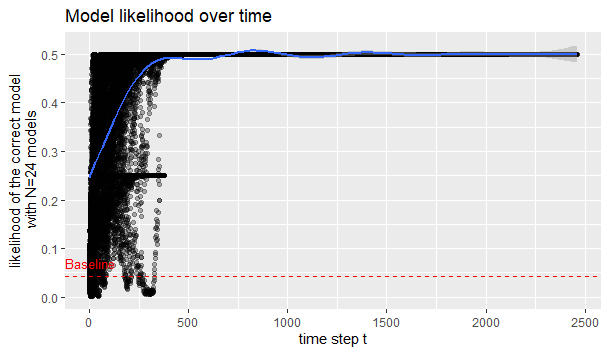
\includegraphics[width=0.95\linewidth]{../../statistics/R_concave_t_likelihoodall_points}
	\caption{Likelihood of the true model over the time steps of the trajectories for Experiment 2b with concave obstacles. The p values are drawn in black, whereas the blue line shows the generalized additive model.}
	\label{fig:rtlikelihoodall}
\end{figure}


\begin{figure}
	\centering
	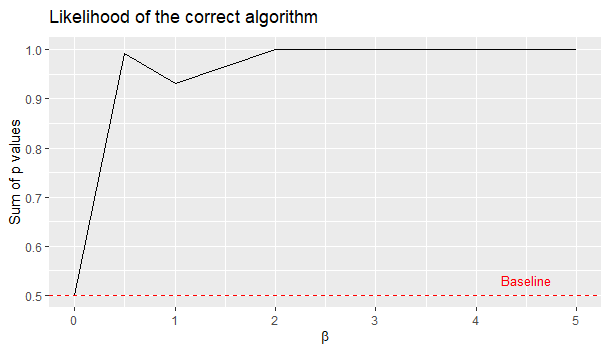
\includegraphics[width=0.95\linewidth]{../../statistics/R_concave_beta_algosum}
	\caption{Likelihood of the correct algorithm in Experiment 2b for all levels of $\beta$, calculated by summing up the p values of all models with the same algorithm as the true model.}
	\label{fig:rbetaalgosum}
\end{figure}

\begin{figure}
	\centering
	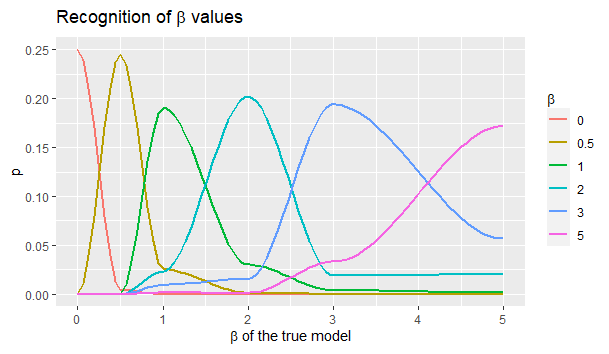
\includegraphics[width=0.95\linewidth]{../../statistics/R_beta}
	\caption{Summarized p values of all model variants with the specific levels of $\beta$ values for Experiment 2b. X axis shows the $\beta$ levels of the true model, colored lines show the local polynomial regression fit of the respective summarized p values of the model variants with specific $\beta$ values.}
	\label{fig:rbeta}
\end{figure}

Likelihoods of the different $\beta$ values relative to the $\beta$ value of the true model can be seen in Figure \ref{fig:rbeta}.


\section{Discussion and Future Work}

As mentioned in the results section, representation types (so a grid-based representation where the agent \textit{knows} its position in the environment versus a vector representation where the agent knows the vector towards its goal) cannot be distinguished in this frame,
as they are isomorphisms and essentially indistinguishable when combined with the way the algorithms work.
This is a very basic issue, and needs to be addressed in any future work on this framework.

Distinguishing the other factors however, algorithm type and $\beta$ values, is working as expected, but could be improved by developing methods to mathematically assimilate the interactions between $\beta$ and algorithm type.
This would make it easier to measure influences of these parameters independently.

Experiment 1 shows that distinguishing between algorithm type in case of the used algorithms is less reliable if no obstacles are present in the environment.
This is to be expected, as both algorithms would choose the direct path to the goal.

The experiments have shown that, as expected, obstacles constituted a problem for the greedy type of algorithm, which can be seen by the high number of necessary steps to reach the goal.
However, the high number of steps in Experiment 2a with the convex obstacle shows that due to the discreteness of the environment, even convex obstacles are a problem to this algorithm.

Recognition of $\beta$ values however works well, especially for Experiments 2a and 2b, as depicted in Figures \ref{fig:rbetaconvex} and \ref{fig:rbeta}.

Future work on this project holds a variety of possibilities.
The first step would be to improve the comparability of models.
There are facets to this: on the one hand, because of the desired and implemented modularity of the modeling approaches, interactions between the modules needs to be explored, 
to achieve meaningful interpretations of a module's details independent of the other modules in a model.

The other side to this is the impact of parameters, such as the determinism factor.
It needs to be explored how to avoid interactions between model specifications and parameter values, in order to be able to draw conclusions on the parameter itself and its effects.
A useful addition to the project for these means, and also for the implementation and development of other or novel approaches, would be a set of baseline experiments translated from real experiments.

From this baseline, other representation and navigation approaches can be explored.
More biologically plausible approaches should be implemented and analyzed, and their interactions studied. For this, existing models and insights from behavioral and neuro-science need to be consulted.

A further possibility would be to integrate a form of ``mental states'' into the models. This could be approached a variety of ways, such as integrating agent states into the environment, or allowing models to be dynamic over time.
The next step would then be to implement inferences to mental states.
E.g., if one wanted to infer whether an agent is in a state of hunger, or infer the amount of exploratory pressure.

Moving on to insect data however needs to include an exploration into as to how far the Markov Property holds for insect movement.
If this is not the case, other forms of problem description need to be taken into account.
A type of memory would in this case be needed, which expands past the heuristic itself.



%\section{Future Work}

\section{Conclusion}

Inverse planning is a viable option for computational research into insect navigation.
It can be used to distinguish between different models, to propose new experiments and to explore latent variables in a computational model.
Representation details, such as memory, can be hypothesized about and compared computationally, forcing model assumptions to be made explicit.
An advantage of using Bayesian methods in this frame is the possibility of conditionality on a variety of parameters, such as goal priors or model priors which could be taken directly from experiments, or hypothesized about to make predictions for future experiments.


%------------- bib --------------------------

\bibliographystyle{apacite}

\setlength{\bibleftmargin}{.125in}
\setlength{\bibindent}{-\bibleftmargin}

\bibliography{pathfinding.bib}

\newpage
\onecolumn
\section*{Appendix}

\subsection{Example 1: Loading experimental data}\label{appendix:ex_loading}
\begin{verbatim}
	# environment definition
	# obstacles can be set, but is not yet supported to be specified in the config within the data file
	obstacles = [(5,5), (6,5)]
	
	# goals and obstacles should be set within the boundaries of the environment as specified in the config
	goals = [Goal('A', (6, 4)), Goal('B', (5, 7))]
	
	# set pixelation if needed
	pix = 2
	
	dm = DataModel("data/example.csv", goals, obstacles, pixelation=pix)

	# goals and obstacles will be translated and scaled to the arena in the model, so if they wish
	# to be used at a later point, they have to be reloaded from the model
	goals = dm.goals
	goalA = goals[0]
	goalB = goals[1]
	obstacles = dm.obstacles
	
	# calculate the optimal policies according to the model
	policies = dm.get_policies()
	
	# calculate the posterior probabilities of the trajectory taken from the file
	posteriors = dm.get_posteriors(policies, dm.trajectory())

	
\end{verbatim}


\subsection{Example 2: Sampling}\label{appendix:ex_sampling}

\begin{verbatim}
	# Specify Environment, lower left corner of the bounding box on the origin
	dims = {'shape': 'Rectangle', 'center_x': 2.0, 'center_y': 2.0, 'grid_width': 4.0, 'grid_height': 4.0}
	goals = [Goal('A', (1, 1)), Goal('B', (3, 3))]
	obstacles = [(1,3), (2,3)]
	
	start_pos = (0, 0)  # any state in the world
	
	# model 1: Vector state, Greedy pathfinding
	model1 = SamplingModel(
		dims,
		goals, 
		obstacles, 
		start_pos, 
		state_type="VectorState", 
		solver="Greedy", 
		determinism=1.0)
	
	# model 2: Grid state, Optimal pathfinding
	model2 = SamplingModel(
		dims, 
		goals, 
		obstacles, 
		start_pos, 
		state_type="GridState", 
		solver="Optimal", 
		determinism=1.0)
	
	policies1 = model1.get_policies()
	policies2 = model2.get_policies()
	
	# choosing the true goal from the list of goals
	true_goal = goals[0]
	
	# sample a trajectory to true_goal according to one model
	sample_trajectory = model1.sample(true_goal)
	
	# calculate the posteriors for both models
	posteriors1 = model1.get_posteriors(policies1, sample_trajectory)
	posteriors2 = model2.get_posteriors(policies2, sample_trajectory)
\end{verbatim}

\end{document}
